% Options for packages loaded elsewhere
\PassOptionsToPackage{unicode}{hyperref}
\PassOptionsToPackage{hyphens}{url}
%
\documentclass[
  9pt,
]{article}
\usepackage{amsmath,amssymb}
\usepackage{lmodern}
\usepackage{iftex}
\ifPDFTeX
  \usepackage[T1]{fontenc}
  \usepackage[utf8]{inputenc}
  \usepackage{textcomp} % provide euro and other symbols
\else % if luatex or xetex
  \usepackage{unicode-math}
  \defaultfontfeatures{Scale=MatchLowercase}
  \defaultfontfeatures[\rmfamily]{Ligatures=TeX,Scale=1}
\fi
% Use upquote if available, for straight quotes in verbatim environments
\IfFileExists{upquote.sty}{\usepackage{upquote}}{}
\IfFileExists{microtype.sty}{% use microtype if available
  \usepackage[]{microtype}
  \UseMicrotypeSet[protrusion]{basicmath} % disable protrusion for tt fonts
}{}
\makeatletter
\@ifundefined{KOMAClassName}{% if non-KOMA class
  \IfFileExists{parskip.sty}{%
    \usepackage{parskip}
  }{% else
    \setlength{\parindent}{0pt}
    \setlength{\parskip}{6pt plus 2pt minus 1pt}}
}{% if KOMA class
  \KOMAoptions{parskip=half}}
\makeatother
\usepackage{xcolor}
\usepackage[margin=1in]{geometry}
\usepackage{longtable,booktabs,array}
\usepackage{calc} % for calculating minipage widths
% Correct order of tables after \paragraph or \subparagraph
\usepackage{etoolbox}
\makeatletter
\patchcmd\longtable{\par}{\if@noskipsec\mbox{}\fi\par}{}{}
\makeatother
% Allow footnotes in longtable head/foot
\IfFileExists{footnotehyper.sty}{\usepackage{footnotehyper}}{\usepackage{footnote}}
\makesavenoteenv{longtable}
\usepackage{graphicx}
\makeatletter
\def\maxwidth{\ifdim\Gin@nat@width>\linewidth\linewidth\else\Gin@nat@width\fi}
\def\maxheight{\ifdim\Gin@nat@height>\textheight\textheight\else\Gin@nat@height\fi}
\makeatother
% Scale images if necessary, so that they will not overflow the page
% margins by default, and it is still possible to overwrite the defaults
% using explicit options in \includegraphics[width, height, ...]{}
\setkeys{Gin}{width=\maxwidth,height=\maxheight,keepaspectratio}
% Set default figure placement to htbp
\makeatletter
\def\fps@figure{htbp}
\makeatother
\setlength{\emergencystretch}{3em} % prevent overfull lines
\providecommand{\tightlist}{%
  \setlength{\itemsep}{0pt}\setlength{\parskip}{0pt}}
\setcounter{secnumdepth}{-\maxdimen} % remove section numbering
\ifLuaTeX
\usepackage[bidi=basic]{babel}
\else
\usepackage[bidi=default]{babel}
\fi
\babelprovide[main,import]{ngerman}
% get rid of language-specific shorthands (see #6817):
\let\LanguageShortHands\languageshorthands
\def\languageshorthands#1{}
\ifLuaTeX
  \usepackage{selnolig}  % disable illegal ligatures
\fi
\IfFileExists{bookmark.sty}{\usepackage{bookmark}}{\usepackage{hyperref}}
\IfFileExists{xurl.sty}{\usepackage{xurl}}{} % add URL line breaks if available
\urlstyle{same} % disable monospaced font for URLs
\hypersetup{
  pdftitle={Pendel},
  pdfauthor={Milena Mensching, Justus Weyers},
  pdflang={de},
  hidelinks,
  pdfcreator={LaTeX via pandoc}}

\title{Pendel}
\author{Milena Mensching, Justus Weyers}
\date{2022-12-12}

\begin{document}
\maketitle

\hypertarget{versuch-1}{%
\section{Versuch 1}\label{versuch-1}}

\hypertarget{thema}{%
\subsection{Thema}\label{thema}}

Bestimmung der Wärmekapazität eines Kaloriemeters. Dieses soll in
Versuch 2 dafür verwendet werden, die spezifische Wärmekapazität zweier
Metalle zu bestimmen.

\hypertarget{versuchsaufbau-und-durchfuxfchrung}{%
\subsection{Versuchsaufbau und
Durchführung}\label{versuchsaufbau-und-durchfuxfchrung}}

\begin{figure}
\centering
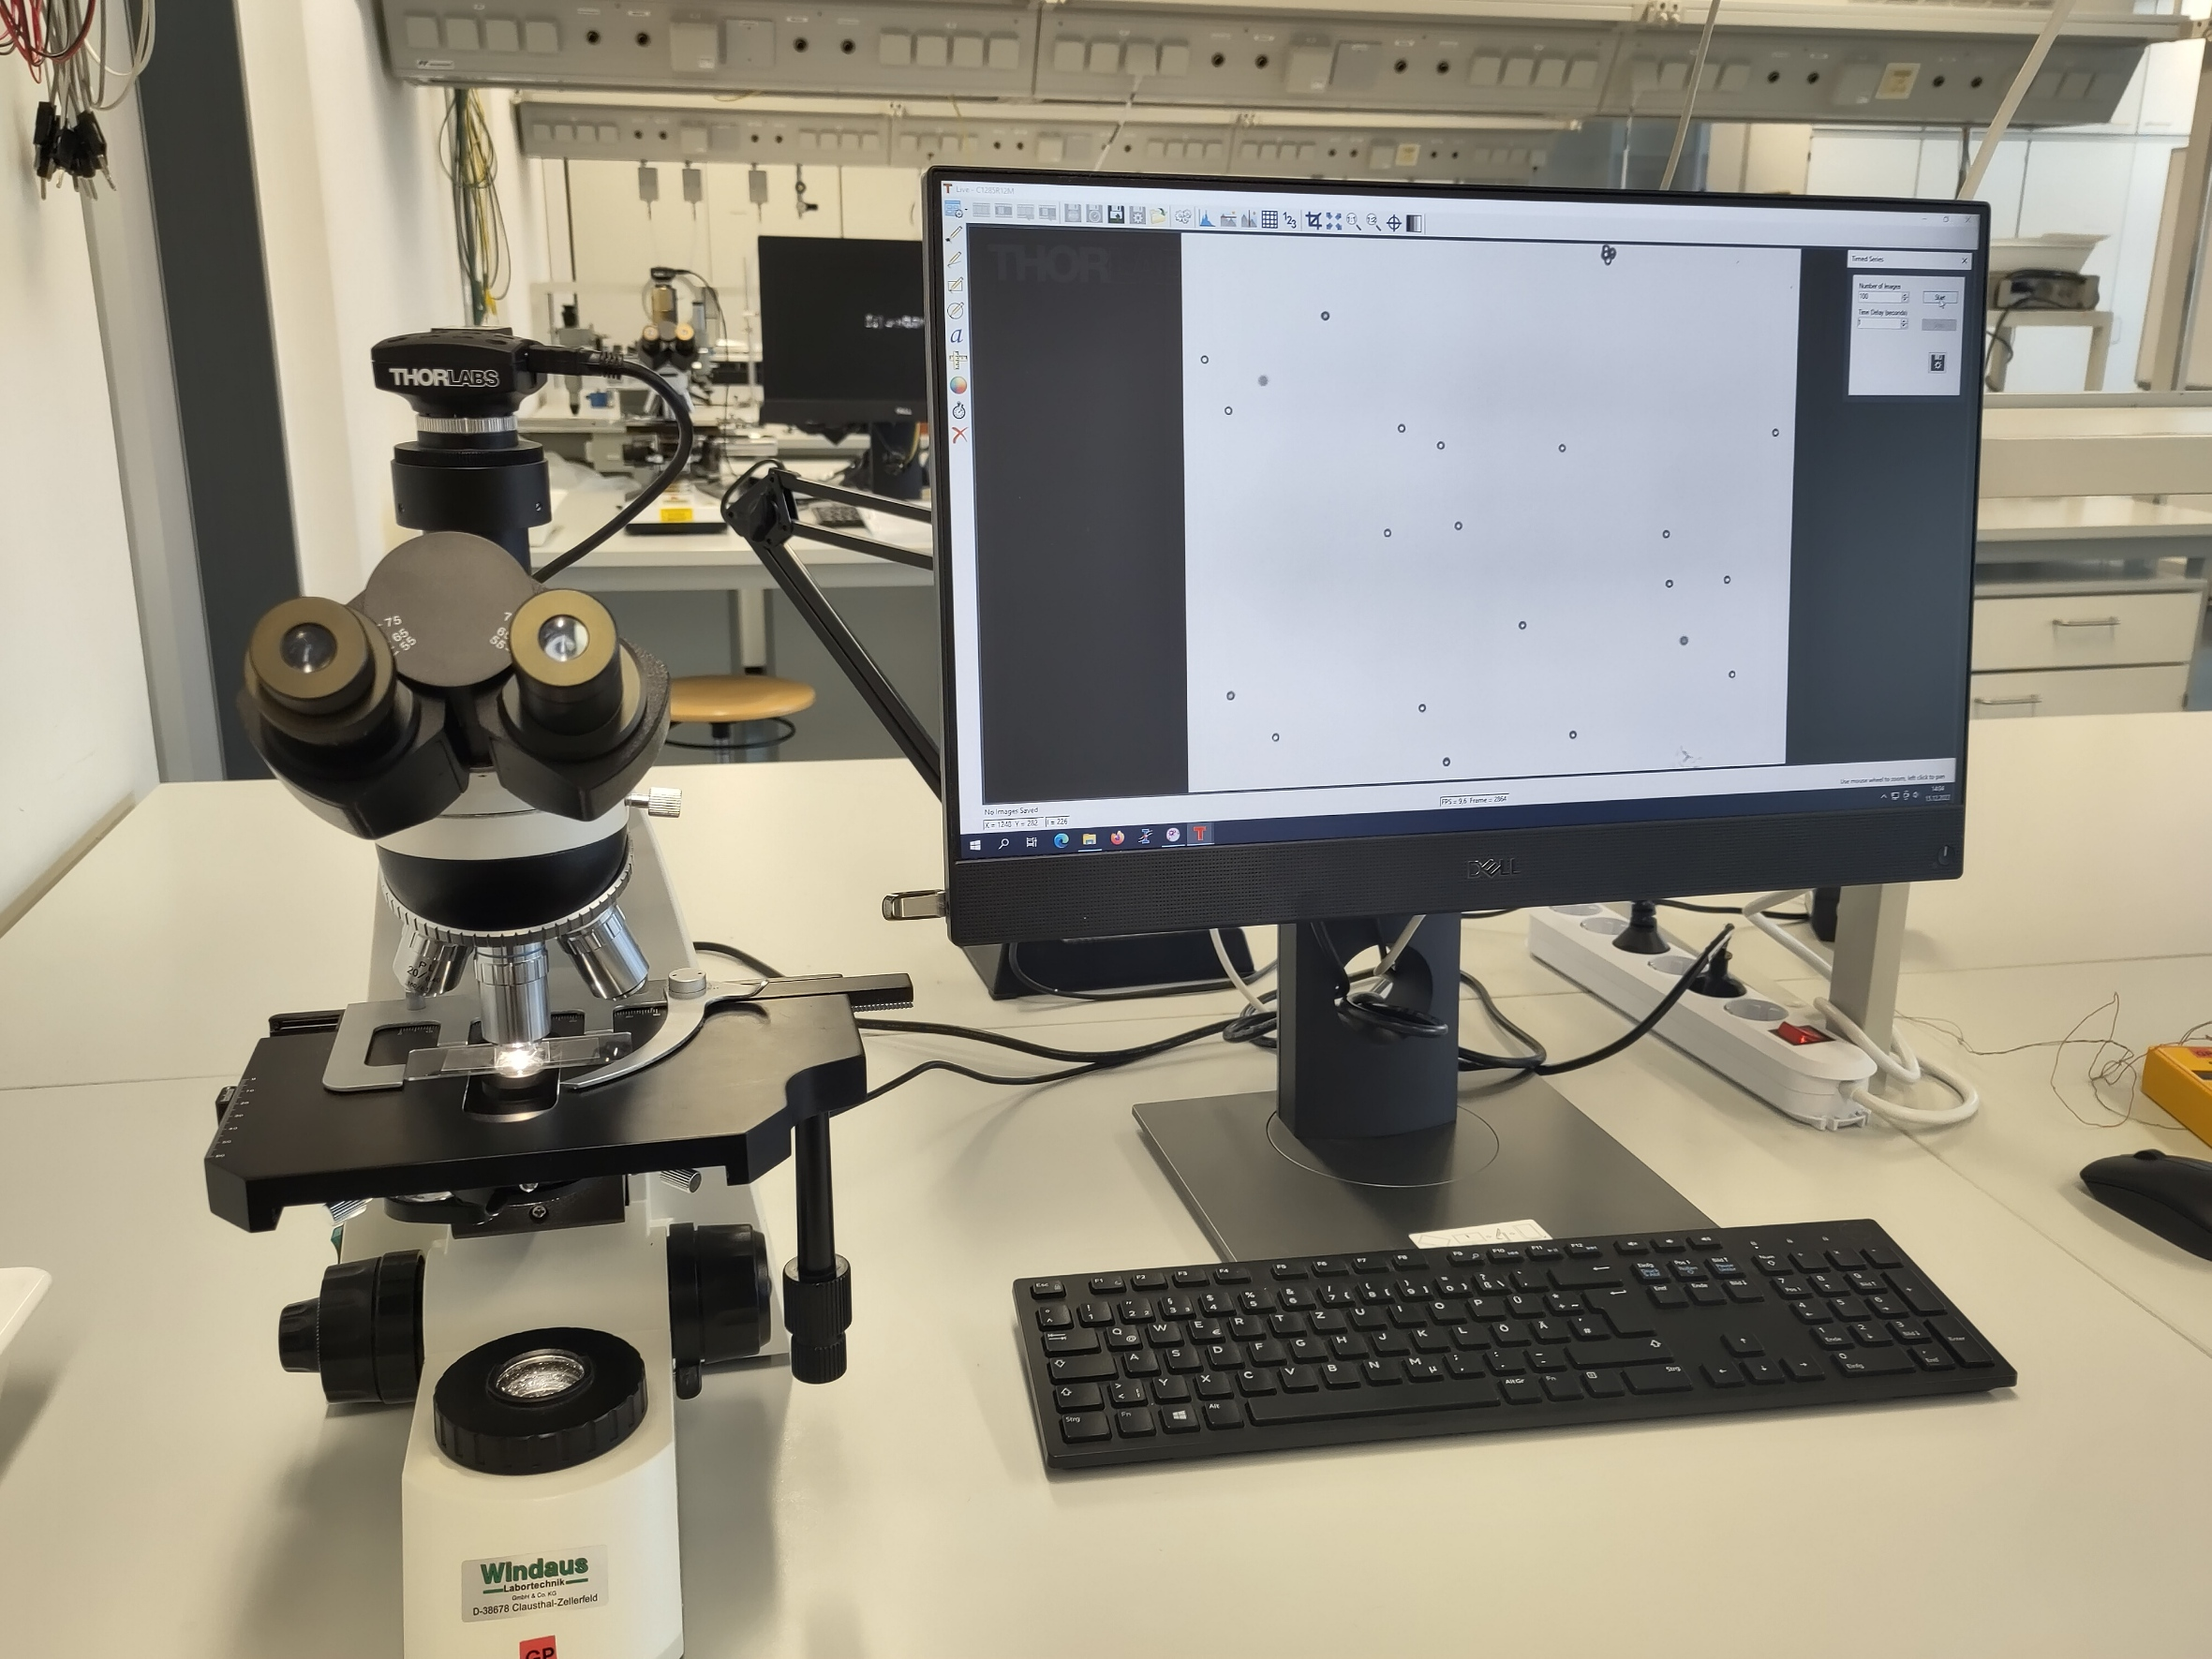
\includegraphics{"Bilder/Versuchsaufbau.png"}
\caption{Versuchsaufbau}
\end{figure}

Zu Beginn des eigentlichen Versuches wird die Raumtemperatur gemessen.

Im Messzylinder werden 100ml und 70 ml Wasser abgemessen und
anschließend in das Kaloriemeter gefüllt. In diesem Zustand wird dessen
Masse gemessen. Der Deckel des Kaloriemeters mit Heizspirale,
Thermometer und Rührstab wird geschlossen. Die Heizspirale wird über
Bananenstecker mit dem AC Netzgerät verbunden. Ein Amperemeter wird in
Reihe und ein Voltmeter parallel geschaltet.

Am Netzgerät wird eine mittlere Leistung eingestellt (50\%) und über den
Zeitraum von sieben Minuten eine Temperatur-Zeit Messreihe aufgenommen.
Während dieser Zeit wird zudem immer wieder die Spannung und die
Stromstärke kontrolliert, die das Kaloriemeter durchfließt
beziehungsweise die an der Heizspirale anliegt.

\hypertarget{fehlerbetrachtung}{%
\subsection{Fehlerbetrachtung}\label{fehlerbetrachtung}}

\hypertarget{beobachtungen}{%
\subsection{Beobachtungen}\label{beobachtungen}}

Die Erhitzung im Kaloriemeter zeigt folgenden Temperaturverlauf:

\begin{verbatim}
## Warning in plot.xy(xy.coords(x, y), type = type, ...): nicht implementierter
## Wert '26' für pch
\end{verbatim}

\begin{figure}

{\centering 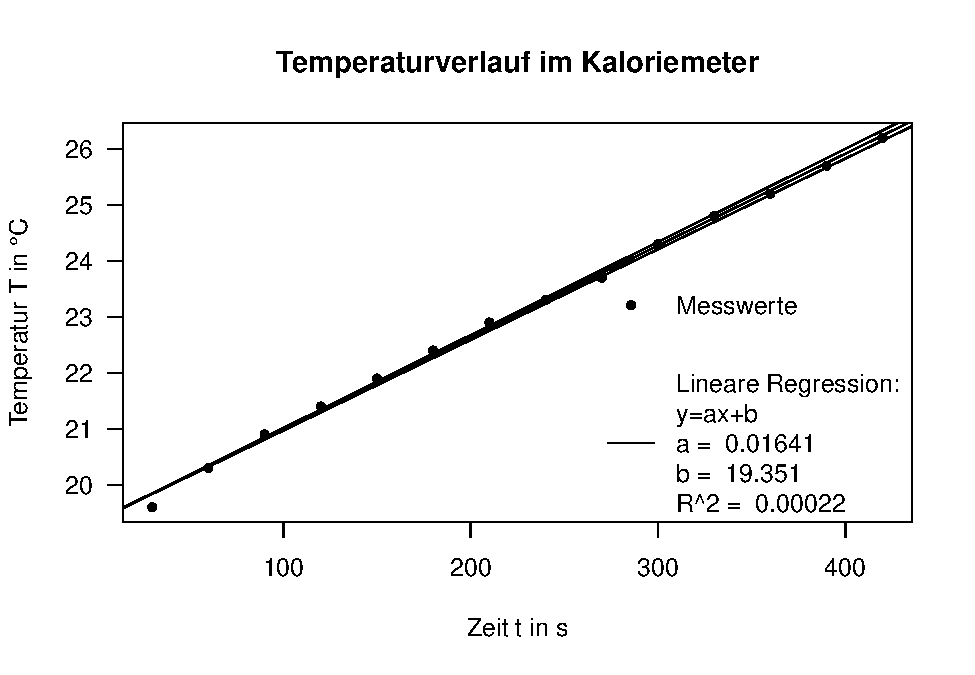
\includegraphics{Kaloriemeter2_files/figure-latex/unnamed-chunk-1-1} 

}

\caption{Testi}\label{fig:unnamed-chunk-1}
\end{figure}

\emph{Abb. 1: Für sieben Minuten wurde der Temperaturverlauf der
Erhitzung des Wassers im Kaloriemeter gemessen}

Der Temperaturverlauf macht im betrachteten Zeitraum einen linearen
Eindruck. Eine Regressionsgerade hat die Steigung
\(a=(1641\pm 22)\cdot 10^{-5}\ ^{\circ} C\ s^{-1}\)

\hypertarget{auswertung}{%
\subsection{Auswertung}\label{auswertung}}

\hypertarget{interpretation}{%
\subsection{Interpretation}\label{interpretation}}

\hypertarget{versuch-2}{%
\section{Versuch 2}\label{versuch-2}}

\hypertarget{thema-1}{%
\subsection{Thema}\label{thema-1}}

\hypertarget{versuchsaufbau}{%
\subsection{Versuchsaufbau}\label{versuchsaufbau}}

\hypertarget{fehlerbetrachtung-1}{%
\subsection{Fehlerbetrachtung}\label{fehlerbetrachtung-1}}

\hypertarget{durchfuxfchrung}{%
\subsection{Durchführung}\label{durchfuxfchrung}}

Im Becherglas wurden für den Versuch ca. \(150ml\) Wasser abgemessen.
Die Bestimmung der verwendeten Wassermasse erfolgte dann durch Abwiegen
des vollen und des leeren Becherglases und durch anschließendes
Subtrahieren der beiden Werte. Die Messunsicherheit der Wassermasse
beträgt zweimal die Skalenunsicherheit der verwendeten digitalen Waage,
also \(u_{m_w}=2*\frac{0,1g}{2\sqrt{3}}=0.058g\).

Die Volumenbestimmung der Metallzylinder erfolgte über die Bestimmung
der Wasserverdrängung in einem Standzylinder. Die Skalenunsicherheit des
Messbechers lag bei \(u_{Skala}=\frac{1ml}{2\sqrt{6}}=0,20ml\).

Nach der Bestimmung des Metallvolumensvolumens und der Größen wurde das
Wasser im Becherglas auf etwa \(50^\circ C\) erwärmt, die genaue
Anfangstemperatur wurde im Kaloriemeter gemessen. Die Skalenunsicherheit
des digitalen Thermometers lag bei
\(u_T = \frac{0.1^\circ C}{2\sqrt{3}} = 0.029^\circ C\). Die gemessene
Anfangstemperatur im Kaloriemeter betrug
\(T_A=(50,000\pm 0,029)^\circ C\).

\hypertarget{beobachtungen-1}{%
\subsection{Beobachtungen}\label{beobachtungen-1}}

Folgendes wurde für das orangene Metall bestimmt: (T\_B (Mischtemp):
(vorläufig 46,1°C) (dann 44,9) (eigeloggt: 44,2))

\begin{longtable}[]{@{}lrlr@{}}
\caption{Aufgenommene Messwerte samt Unsicherheiten für das untersuchte
orangene Metall}\tabularnewline
\toprule()
& Messwert & Geräteart & Unsicherheit \\
\midrule()
\endfirsthead
\toprule()
& Messwert & Geräteart & Unsicherheit \\
\midrule()
\endhead
Becherglas mit Wasser {[}g{]} & 235.5 & digital & 0.029 \\
Masse Becherglas {[}g{]} & 97.4 & digital & 0.029 \\
Wassermasse {[}g{]} & 138.1 & - & 0.058 \\
Metallvolumen {[}cm³{]} & 23.0 & analog & 0.200 \\
Anfangstemperatur {[}°C{]} & 50.0 & digital & 0.029 \\
Mischtemperatur {[}°C{]} & 44.2 & digital & 0.029 \\
\bottomrule()
\end{longtable}

Folgendes wurde für das graue Metall bestimmt: (T\_B (Mischtemp):
(vorläufig 44,1°C) (dann 43,4) (eigeloggt 42,8))

\begin{longtable}[]{@{}lrlr@{}}
\caption{Aufgenommene Messwerte samt Unsicherheiten für das untersuchte
graue Metall}\tabularnewline
\toprule()
& Messwert & Geräteart & Unsicherheit \\
\midrule()
\endfirsthead
\toprule()
& Messwert & Geräteart & Unsicherheit \\
\midrule()
\endhead
Becherglas mit Wasser {[}g{]} & 241.3 & digital & 0.029 \\
Masse Becherglas {[}g{]} & 97.4 & digital & 0.029 \\
Wassermasse {[}g{]} & 143.9 & - & 0.058 \\
Metallvolumen {[}cm³{]} & 22.0 & analog & 0.200 \\
Anfangstemperatur {[}°C{]} & 49.1 & digital & 0.029 \\
Mischtemperatur {[}°C{]} & 42.8 & digital & 0.029 \\
\bottomrule()
\end{longtable}

\hypertarget{auswertung-1}{%
\subsection{Auswertung}\label{auswertung-1}}

\hypertarget{interpretation-1}{%
\subsection{Interpretation}\label{interpretation-1}}

\end{document}
